% Activate the following line by filling in the right side. If for example the name of the root file is Main.tex, write
% "...root = Main.tex" if the chapter file is in the same directory, and "...root = ../Main.tex" if the chapter is in a subdirectory.
 
%!TEX root =  mainMastersProject.tex

\chapter[Simple Spatial Simulations]{A Simple Robbery - Spatial Simulations and their Bayesian Networks}

Three experiments: 1) getting the bayesian networks with decreased precision by disturbing the cpts 2) testing the effect of a simulation parameter change on the BN (how different does it become. 3) investigating the effect of hidden information/private knowledge on the network.
Summary:

 The problem is that in the previous chapter, we have established that we have a method to convert a simple, forward chaining simulation, to a collection of data, which then in turn can be used to create a Bayesian Network, that represents the situation in the simulation relatively well (some problems none-withstanding, accuracy and RMS error are generally ok even in increments that people might plausibly be able to estimate ~ intervals of 0.33/0.25-ish). However, this was totally 100\% determined by deterministic forward chaining rules. The real world does not run on deterministic forward chaining rules (as far as we know). At least, we are spatially situated, which means that there are probabilities that will arise out of interactions between agents and their environment. These probabilities are not `set' in the same ways as the probabilities are set in the previous chapter, they arise organically from interactions: eg: an agent has to be located at a door to break in, an agent can be seen by a camera only in some locations of the simulation. We do not know these probabilities a-priori (although we can probably calculate them, I don't know).
 
New idea: We create spatially situated simulations that are more complex, and see if they work the same way/are as accurate \& rms as the previous. Then we will also use these simple spatial simulations to test two hypotheses about 1) the effect of private knowledge and 2) the effect of parameters.


\section{Experiment 1: Generating BNs with disturbances}

In this first experiment, I will be creating an agent simulation of a very simple crime case. I will run the simulation for some number of times, and then automatically generate BNs, based on the K2 algorithm. Then I will change the values of the cpts in the BNs, to see if we can accurately predict the outcome even with low precision in cpts, given the structure of the BN.

\subsection{Introduction}

The scenario that the agents play out goes as follows. There are two agents. They are neighbors. One day, the agent who lives in the house on the right ($R$), walks past the house of the other agent ($L$). $R$ looks inside, if it can. Sometimes it cannot look inside, because $L$ has drawn the curtains. However, if $R$ can look inside, it might see a goodie in the house. It also might not see a goodie, if $L$ has lost the goodie - in that case, the goodie has been lost. However, if the goodie is there, $R$ will know that the goodie is there. Then, because $R$ is a rational agent, it will try to calculate the worth of the object, and if it might want to steal it. It can decide to target the object. If $R$ knows and targets the object, $R$ has a motive. Then, $R$ attempts to break into the house by breaking the lock on the door, grabbing the goodie, and running away to its own house.  Meanwhile, $L$ is returning home. If $R$ thinks that $L$ might have seen it stealing, $R$ will flee home, with or without the goodie. $L$ has also hung up security cameras on the outside corner of its house, that might serve as evidence against $R$.

With regards to the end, there can be three outcomes: either the goodie is lost, the goodie is not lost but was stolen successfully, or the goodie is not lost and wasn't stolen successfully. %({\color{red}does this mean that there was always a stealing attempt? check in jup}). 
The environment of the agents is very simple, just two `houses' (rectangles, really). The environment and the agents (with their vision parameter) are shown in Figure~\ref{env}.

\begin{figure}[htbp]
\begin{subfigure}{.5\textwidth}
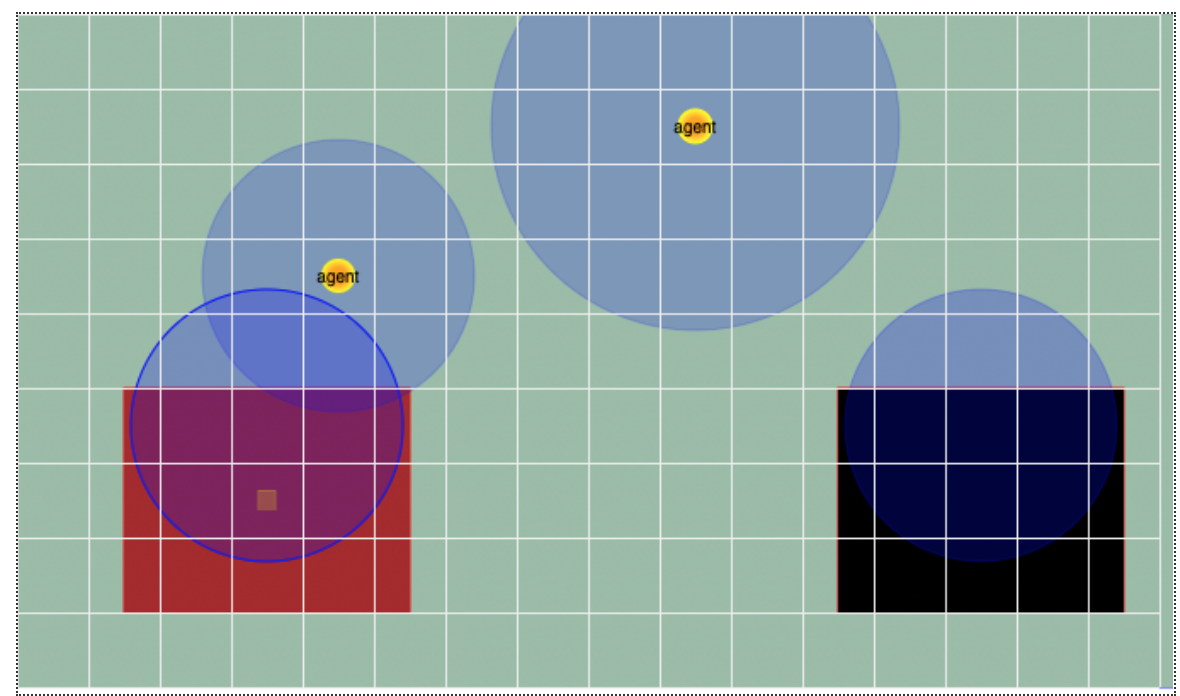
\includegraphics[width=\linewidth]{images/sim1.png}
\caption{The simulation with the 2 agents.}
\end{subfigure}
\begin{subfigure}{.5\textwidth}
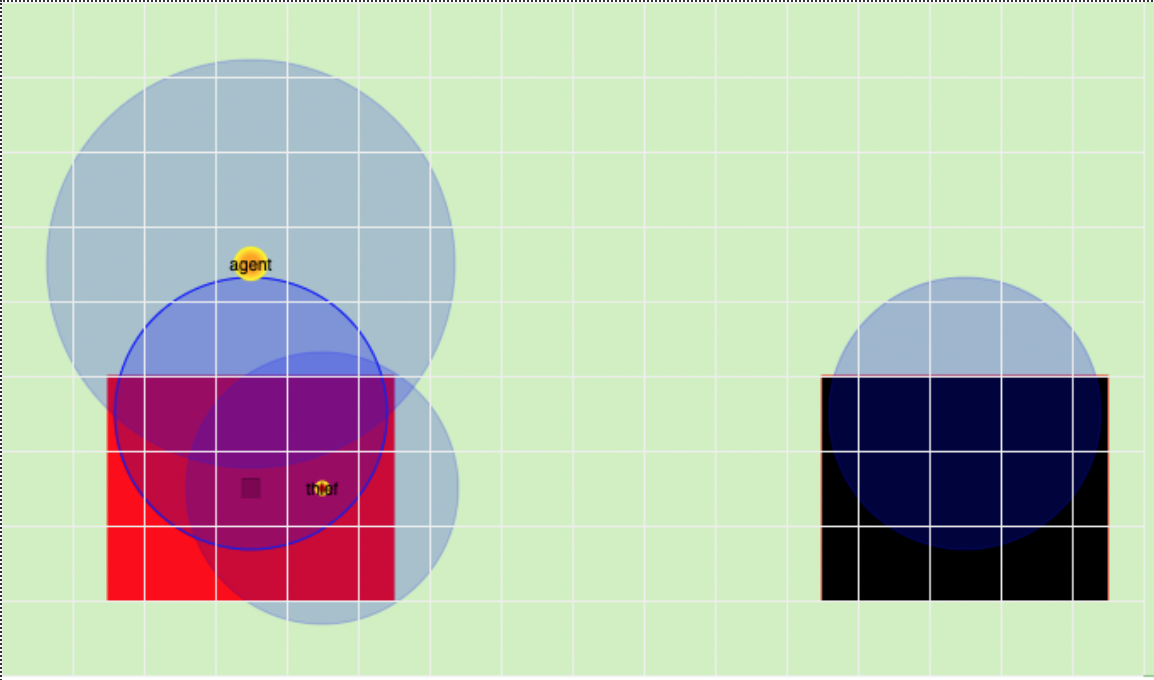
\includegraphics[width=\linewidth]{images/stealing.png}
\caption{The agent attempts to steal something but flees when it thinks that it is noticed.}
\end{subfigure}
\caption{Agents behaving badly in simulation.}
\label{env}
\end{figure}

\subsection{Methods}
There are four things to be explained here: the agent behaviour, the operationalisation of the random variables, the simulation (meta-)parameters, and the process through which the cpts of the given BN is to be disturbed.

\subsubsection{Agent behaviour}
flowchart here.

\subsubsection{Operationalisation of the RVs}

The operationalisation of the random variables is very important. In the table below are all the reporters and how they are defined.

\begin{adjustbox}{center}
\footnotesize
\centering
\begin{tabular}{|l|l|}
 \hline
 RV &Operationalization\\
 \hline
lost\_object   & A random number generator (0, 1) generates a number. If the number $\leq 0.2$, the object is lost.\\
curtains & A random number generator (0, 1) generates a number. If the number $\leq 0.8$, the house has no curtains.  \\
raining & A random number generator (0, 1) generates a number. If the number $\leq 0.5$, it is raining.   \\
know\_object & if we see an object in our vision that is not our own, and we are not already targeting some`
thing else  \\
target\_object & if we know the object exists, and we consider the value of the object higher than our risk threshold.  \\
motive & if we have a target \\
compromise\_house & if we are adjacent to the target's house's door, and we have a breaking and entering skill of greater than 5. \\
flees\_startled & if we see another agent and we haven't been observed yet  \\
successful\_stolen & if we're not in someone's house anymore and we have the object in our possession \\ 
E\_s\_spotted\_by\_house&  {\color{red} todo fill in}. \\ 
E\_disturbed\_house&   \\ 
E\_object\_is\_gone&   \\ 
E\_broken\_lock&   \\ 
E\_s\_spotted\_with\_goodie&   \\ 
E\_private&   \\ 
\hline
\end{tabular}
\end{adjustbox}

\subsubsection{Simulation parameters}
Number of runs: 1000

\subsubsection{Disturbing the cpts}
We generated only one Bayesian Network, with the data we collected from the simulation. Then, we create many new networks, with this network as a basis. We do not change the number of nodes (we do not leave out or add nodes), nor the structure of the Bayesian network. We only change the values in each node's conditional probability table (cpt). In this case, we round the values in the cpt's, such that the BN becomes increasingly less precise. The intuition behind this is, that when expert users are going to elicit the probabilities, we do not know how robust the network is against smaller and larger imprecisions in the elicited probabilities. By simulating such imprecisions, we can compare the accuracy and rmsq error of the more imprecise networks to the ground truth of the `real' network. 

We round every value in the cpts $c$ to each of $i, i \in \{\text{no disturbance}, 0.05, 0.1, 0.125, 0.2, 0.25, 0.33, 0.5\}$, according to \[ floor(\frac{c}{i} + 0.5) \cdot i.\]



\subsection{Results}

See Figure~\ref{laptop}


\begin{figure}[h]
\begin{center}
\begin{subfigure}{.7\textwidth}
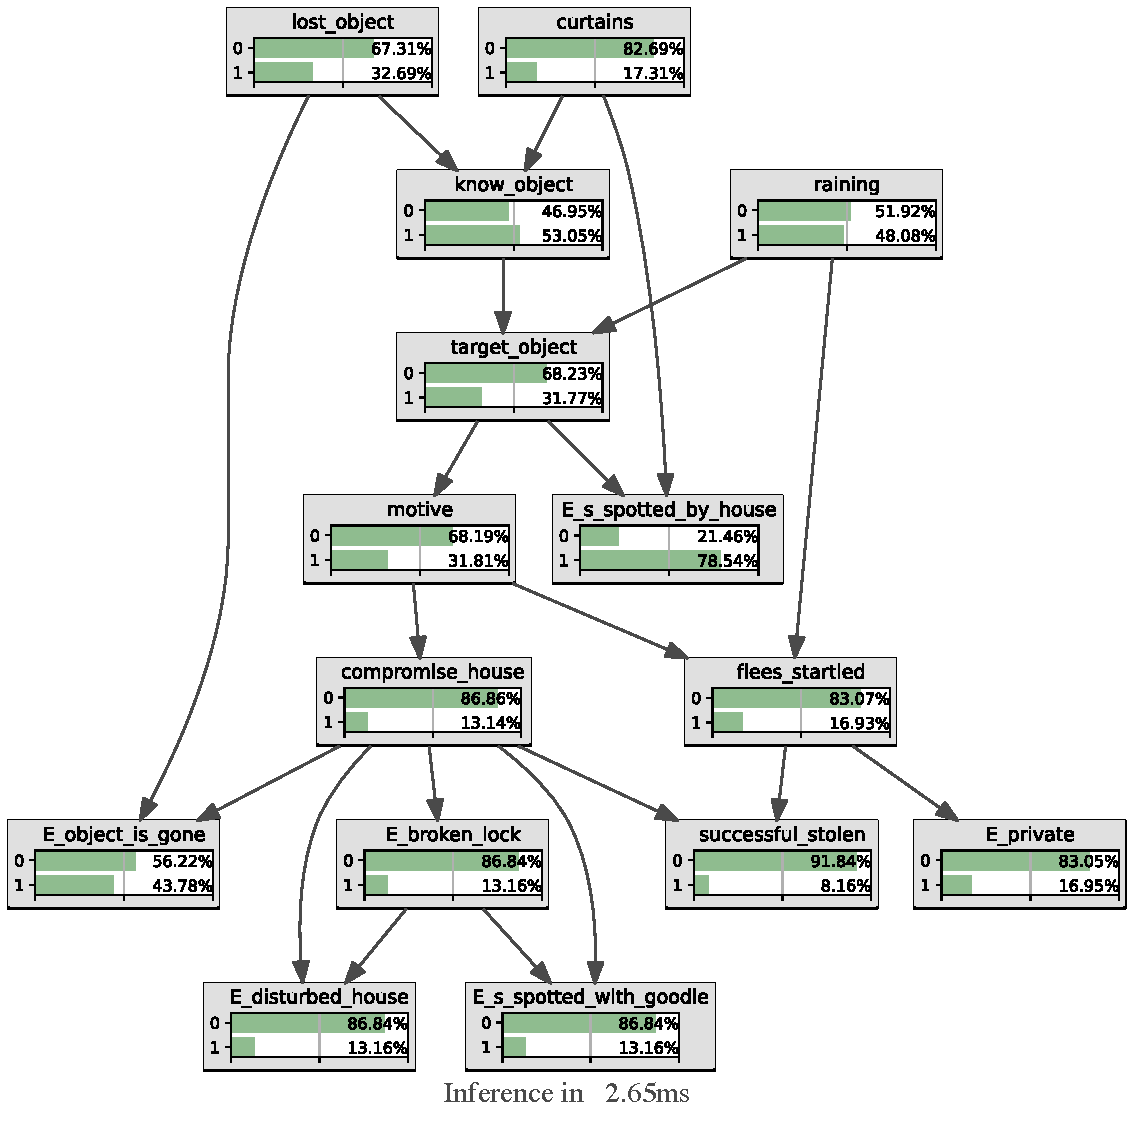
\includegraphics[width=\linewidth]{../experiments/StolenLaptop/bnImage/BNIMAGEStolenLaptop.pdf}
\caption{network structure}
\label{laptopAcc}
\end{subfigure}
\end{center}

\begin{subfigure}{.5\textwidth}

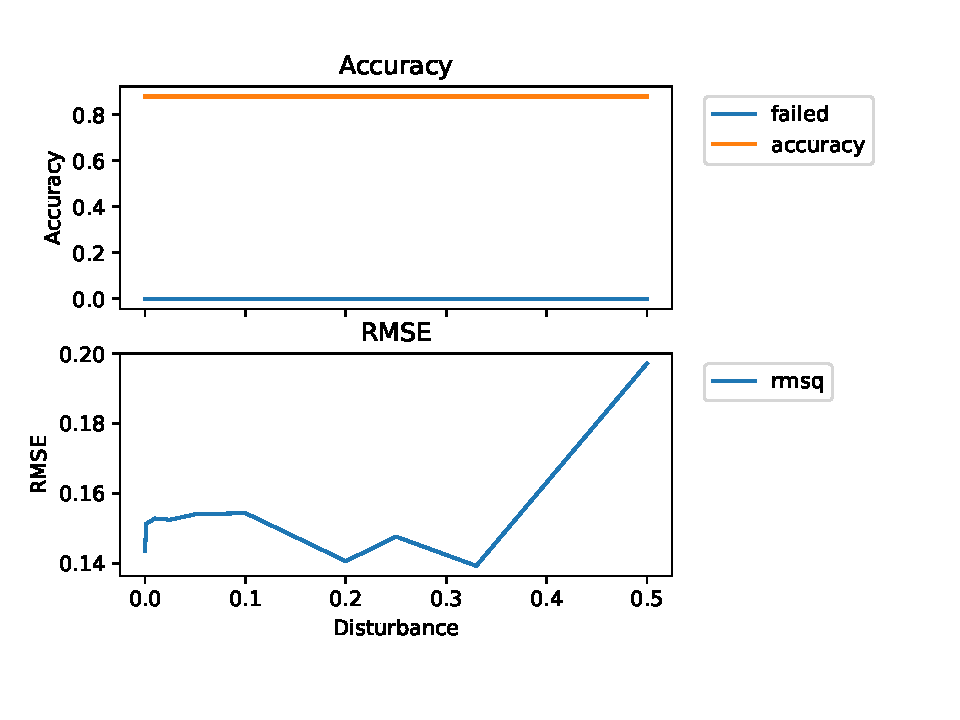
\includegraphics[width=\linewidth]{../experiments/StolenLaptop/plots/performance_StolenLaptop.pdf}
\caption{Accuracy (100\% to 0\%) and Root Mean Square error (1 - 0) }
\label{laptopAcc}
\end{subfigure}
\begin{subfigure}{.5\textwidth}

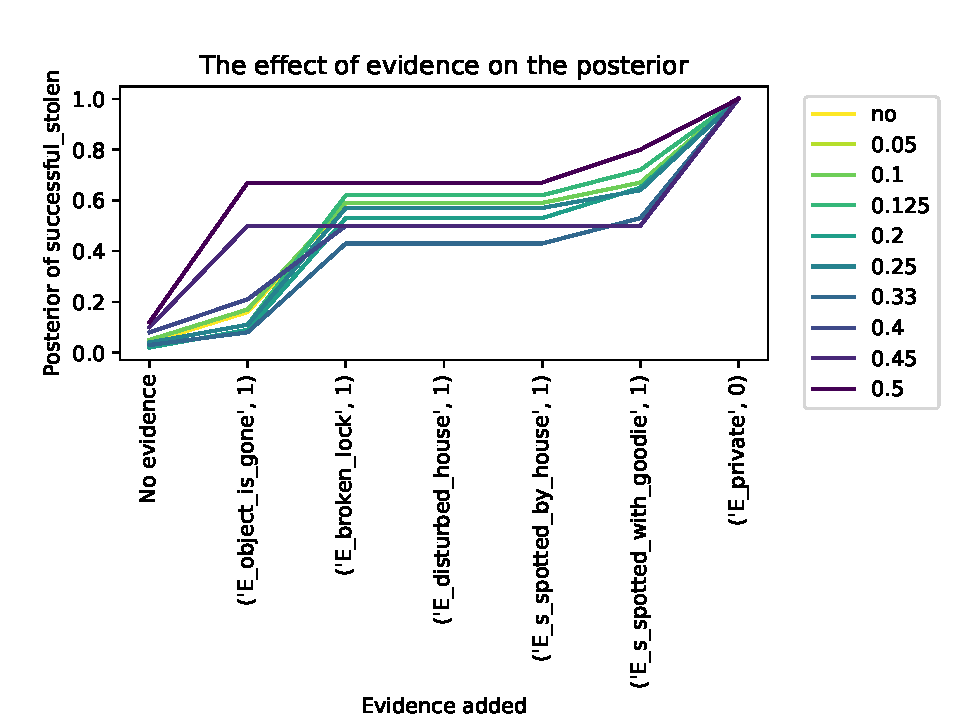
\includegraphics[width=\linewidth]{../experiments/StolenLaptop/plots/posterior_StolenLaptop.pdf}
\caption{effect of evidence on posterior}
\label{laptopPosterior}

\end{subfigure}
\caption{The network, the accuracy and root mean square for rounding the cpts to intervals, and the effect of evidence on the posterior for stolen laptop simulation.}
\label{laptop}
\end{figure}


%\begin{figure}[h!]
%\begin{center}
%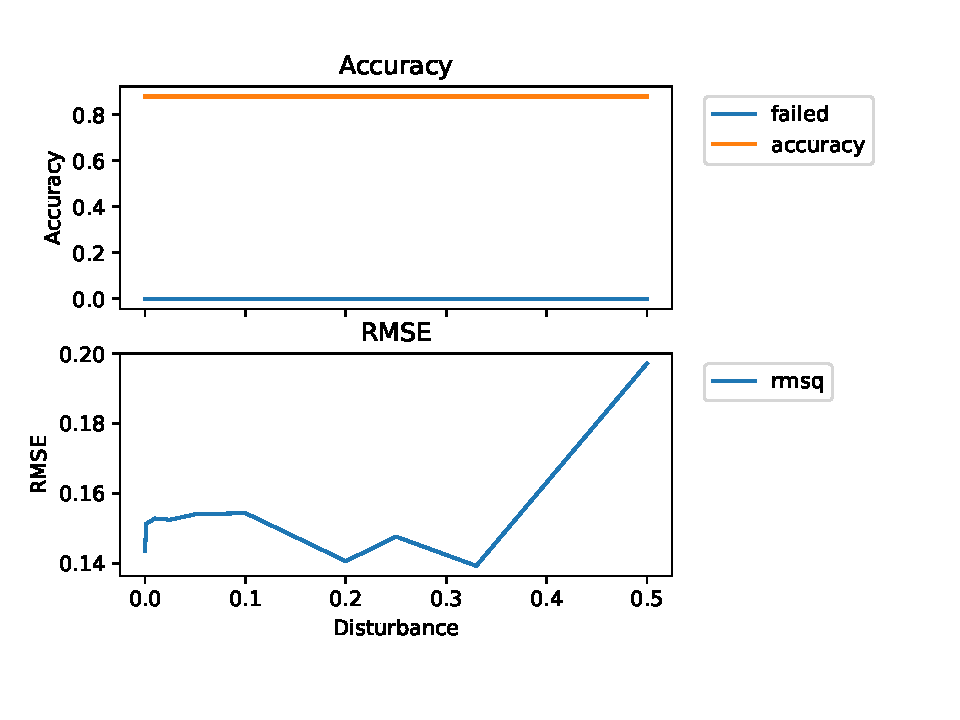
\includegraphics[]{../experiments/StolenLaptop/plots/performance_StolenLaptop.pdf}
%\caption{Accuracy (100\% to 0\%) and Root Mean Square error (1 - 0) for rounding to different intervals in stolenLaptop network and simulation}
%\label{laptopAcc}
%\end{center}
%\end{figure}



Overall pretty accurate. This shows that small disturbances in rounding - and even larger disturbances in rounding, such as to 0.25 or even 0.33, does not matter very much for the accuracy of this specific network. 

{\color{red} todo: add automatic table with accuracies and rms generated}.


\subsection{Discussion}

The network itself makes sense. The spurious node `raining' is not connected to any other node, because the rain should not affect what happens.

The fact that these networks can be rounded without losing accuracy, means that even with a lack of precision in the ctps of the network, the network is still able to accurately predict outputs - eg, whether a node is going to be true or false given a set of evidence. Changing the precision of the network does not change the network structure itself, this is kept constant - it is generated first, and then the cpts are rounded to arbitrary intervals. 

This shows that even when this network's cpt's only contain probability values, [0, 0.33, 0.66, 0.99], we still get the reflection of the evidence in the network. 

\subsubsection{Network structure}

Problem: the disturbance of the cpts means that we're only disturbing the cpts, and not the structure of the network itself. If we look at the ordering of the non-evidence nodes in the network, then we can see that they are ordered temporally - parent nodes happen before child nodes. However, there are many sibling-nodes (nodes with the same parents), and how these nodes relate to each other temporally cannot be understood from the BN alone (does compromise house come before or after flees startled?). 

Knowing to which parent node some pieces of evidence should connect is also not straightforward: evidence could connect to more or fewer parent nodes than they are now. Due to the limitations of the K2 algorithm, I'm not sure if we can create a rule where evidence only connects to one parent.





\section{Experiment 2: Investigating Evidence Strength.}


\subsection{Introduction}
A funny thing is that this simulation we can test how the evidence strength is dependent on certain parameters in the network. For a simple example, see the radius of camera vision. If we have the Reporter ``agent seen near house''/"agent spotted by camera", and by that we mean, that if the agent is visible in the camera placed near the house, then the range of vision of the camera becomes relevant for the investigation. If the camera is super good and can see the agent even when he's not near the house, then the effect of being-seen-on-camera should decrease: it becomes less relevant that the agent was seen by the camera, because they usually are. On the other hand, if the camera is pointed only at the door, then being seen by the camera is relevant, the agent is only by the door when he's trying to break in. Below you see a plot of camera vision range vs effect on posterior when the node is turned on (given the same structure of the BN).

\subsection{Methods}
I changed the parameter of vision of the camera for the simulation between 1 and 15, for the rest the simulation was the exact same. I didn't apply any disturbances to the network.

\subsection{Results}

See Figure~\ref{vision}

\begin{figure}[h]
\begin{center}
\begin{subfigure}{.7\textwidth}
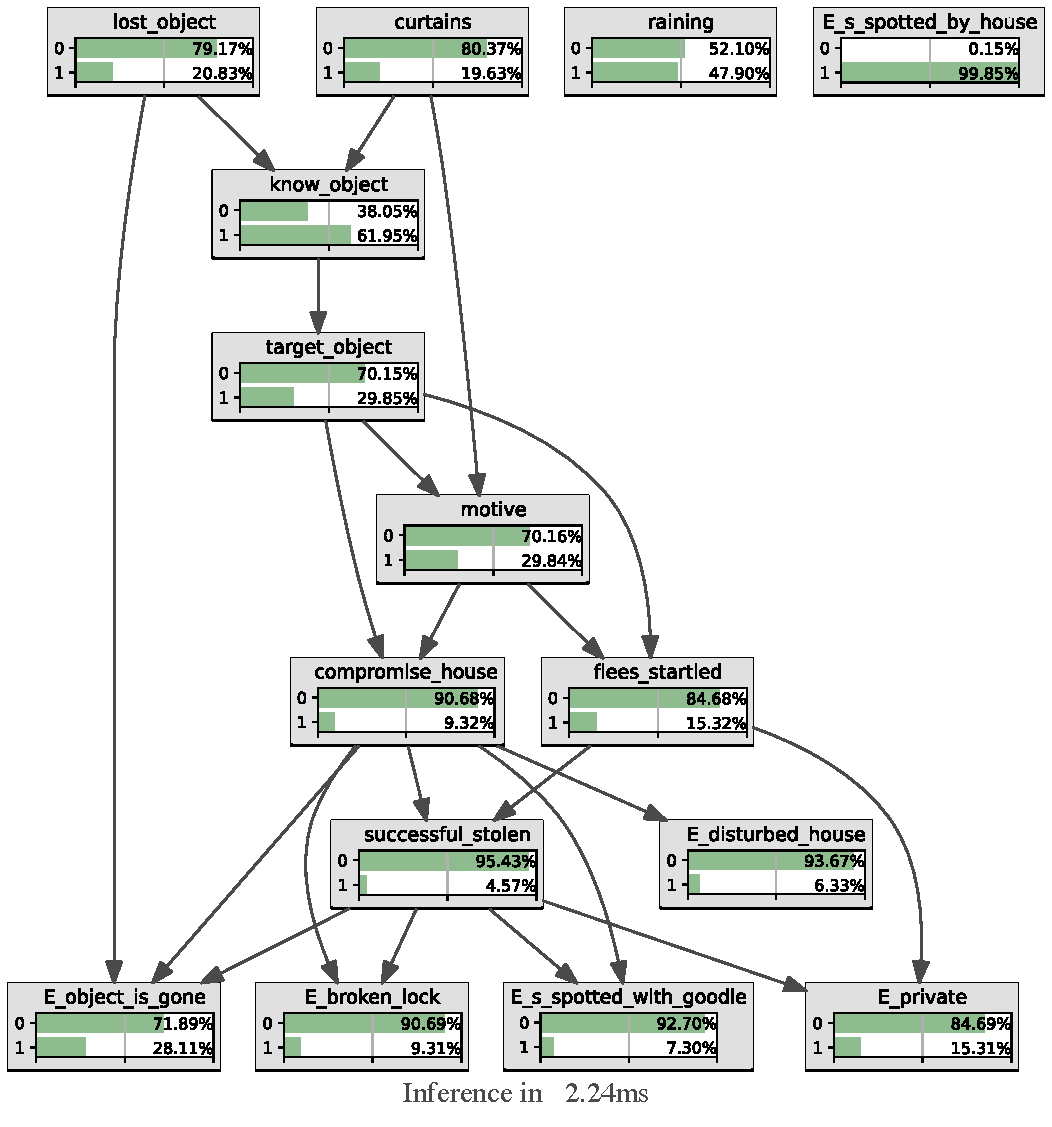
\includegraphics[width=\linewidth]{../experiments/StolenLaptopVision/bnImage/BNIMAGEStolenLaptopVision.pdf}
\caption{network structure}
\label{visionlaptopAcc}
\end{subfigure}
\end{center}

\begin{subfigure}{.5\textwidth}

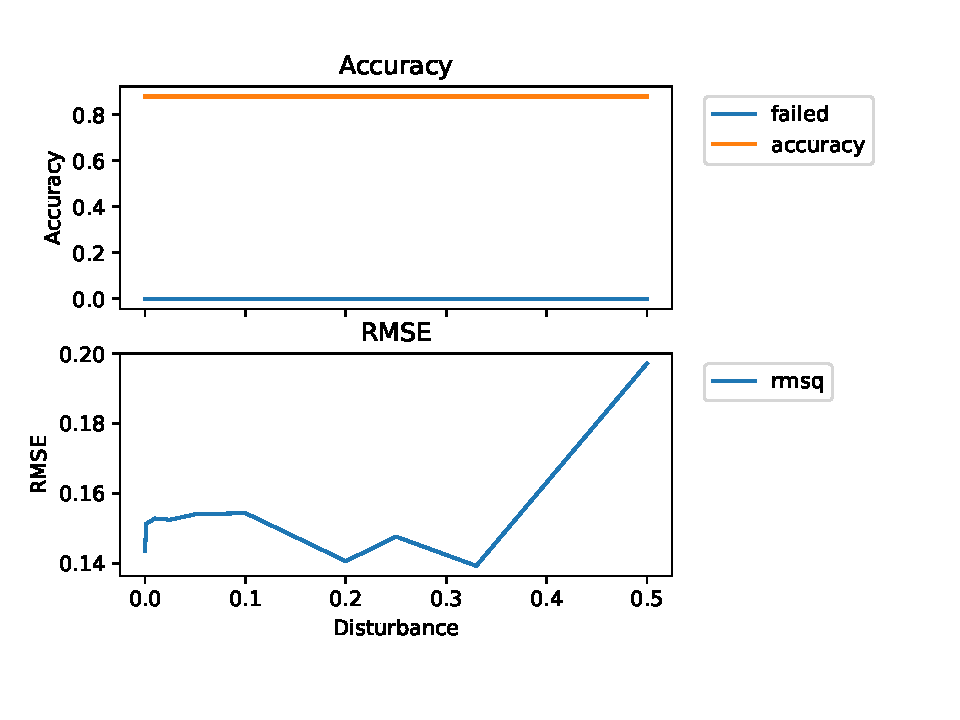
\includegraphics[width=\linewidth]{../experiments/StolenLaptop/plots/performance_StolenLaptop.pdf}
\caption{Accuracy (100\% to 0\%) and Root Mean Square error (1 - 0) }
\label{laptopAcc}
\end{subfigure}
\begin{subfigure}{.5\textwidth}
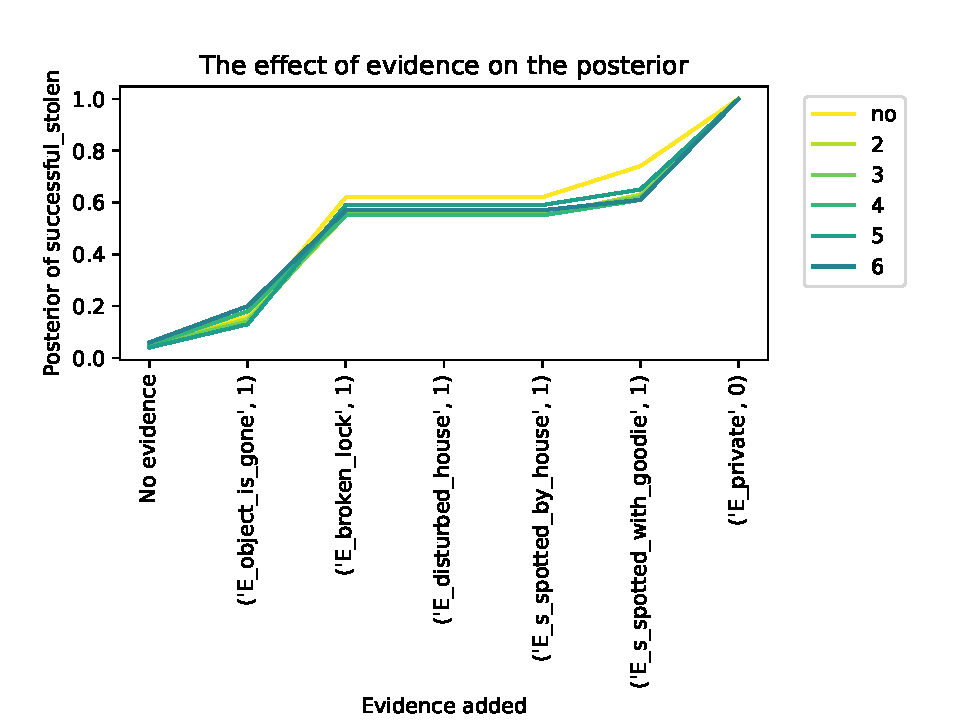
\includegraphics[width=\linewidth]{../experiments/StolenLaptopVision/plots/posterior_StolenLaptopVision.pdf}
\caption{effect of evidence on posterior}
\label{visionlaptopPosterior}
\end{subfigure}
\caption{The network, the accuracy and root mean square for rounding the cpts to intervals, and the effect of evidence on the posterior for stolen laptop simulation.}
\label{vision}
\end{figure}



\subsection{Discussion}
We see here, that the name of the variable is actually incorrect. It shouldn't be called "agent seen near house", because the reporter is not actually reporting that the agent is near the house - instead it is reporting whether the agent is within the vision of the camera. So properly it should be called "agent is seen in camera", or we can rewrite the reporter to measure whether the agent is actually near the house. 

But, this means that the BN is not responsive to the effect of relevance in the real world. 


\section{Experiment 3: Investigating Private Knowledge}

\subsection{Introduction}
The most obvious problem in crime is the distribution of knowledge. The criminal will (usually) know what he did, victims can testify, the police knows something else. Etc. So our ultimate goal is just to collect all the private knowledge of all the people involved, and paint a collective knowledge picture that (ideally) everyone can agree on, and then the judge can decide. Of course, it is not in the interest of everyone to freely share their private knowledge all the time. Police might not want to talk about the limitations of their evidence (or their ways of procuring it), witnesses and victims might not want to talk due to incrimination, guilt/shame or relations to the people involved, and suspects might not want to share their murder plans (obviously). So there's so much private knowledge, and our Bayesian Network assumes that we can just get into the heads of everyone and report on what we find there. So what if we cannot? What if we lose some information - like that of the suspect: that the suspect will flee if it thinks that it is being observed?

\subsection{Method}
Drop column Private knowledge and evidence for it, see the effect on the posterior. See the effect on the disturbances.


\subsection{Results}


See Figure~\ref{private}

\begin{figure}[h]
\begin{center}
\begin{subfigure}{.50\textwidth}
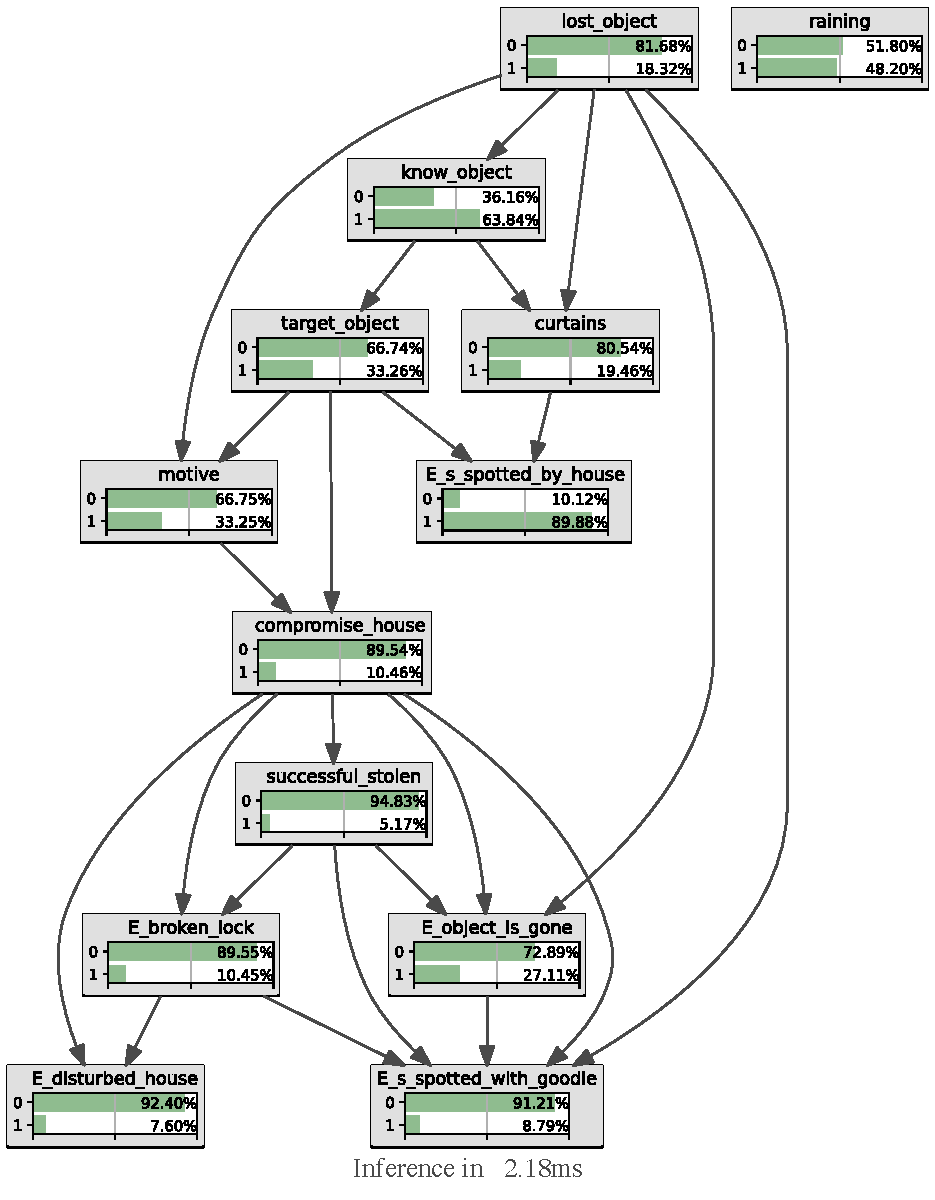
\includegraphics[width=\linewidth]{../experiments/StolenLaptopPrivate/bnImage/BNIMAGEStolenLaptopPrivate.pdf}
\caption{network structure}
\label{privatelaptopAcc}
\end{subfigure}
\end{center}

\begin{subfigure}{.45\textwidth}
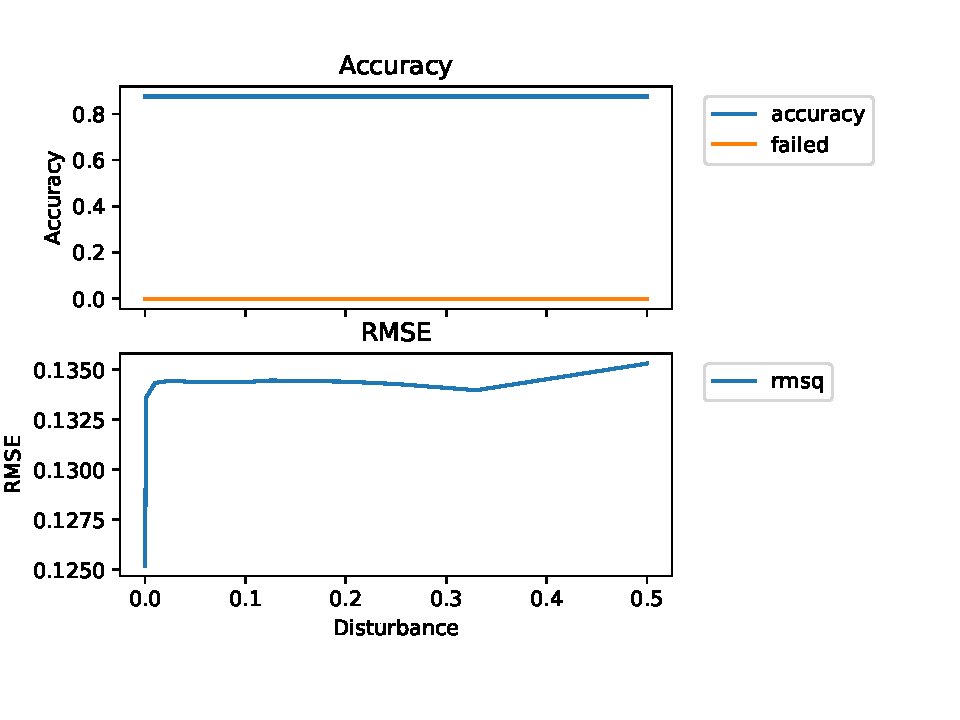
\includegraphics[width=\linewidth]{../experiments/StolenLaptopPrivate/plots/performance_StolenLaptopPrivate.pdf}
\caption{Accuracy (100\% to 0\%) and Root Mean Square error (1 - 0) }
\label{privatelaptopAcc}
\end{subfigure}

\begin{subfigure}{.45\textwidth}
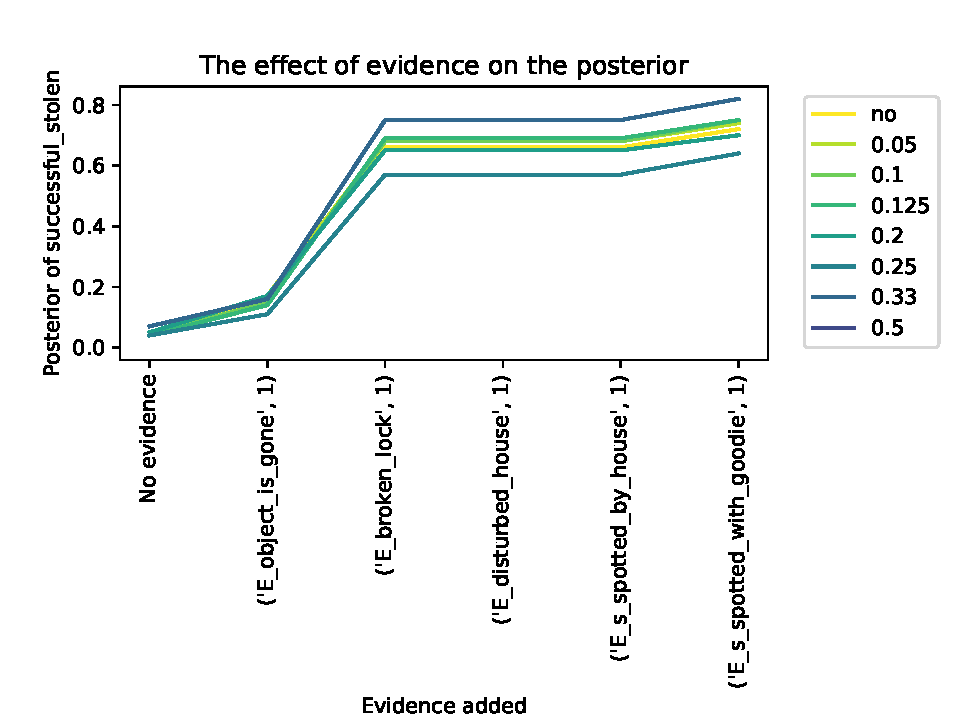
\includegraphics[width=\linewidth]{../experiments/StolenLaptopPrivate/plots/posterior_StolenLaptopPrivate.pdf}
\caption{posterior }
\label{privatelaptoppost}
\end{subfigure}

\caption{The network, the accuracy and root mean square for rounding the cpts to intervals, and the effect of evidence on the posterior for stolen laptop simulation.}
\label{private}

\end{figure}


\subsection{Discussion}

Seems to be effective, posterior never goes to 1. Lack of private knowledge hence will affect the end results, even if it will not affect the trajectory of the evidence progression. Overall accuracy and rms performs worse as well.


\section{Conclusion}


{\color{blue} TLDR: We can build an accurate network for a spatial simulation, even when we disturb the cpts. We can see how the posterior probability of an outcome becomes more likely when we add incriminating evidence. We can change parameters in the simulation (change vision radius of camera) and this effects the network (nodes do not show up). We can remove private knowledge, and this reduces the overall accuracy of the network from 100\% to 80\%, although it does not change the `shape' of the effect of the other evidence on the posterior. This all needs to be worked out.}


Simulating works, accuracy and RMS fine.

Table of accuracies and rms for the three experiments for comparisons.

We run into problems when we use words like `near' in our node names. We're lucky that we know what we mean (because our reporter forces us to make this explicit). We do not just ground the probabilities in our network, but we actually also ground our random variables - we have a measure of exactly what events we are interested in, and which we aren't.

We are in trouble with private knowledge, dropping this column from our table (which means that we don't know it) when we make our BN, we're drastically reducing our uh. Accuracy, and increasing our RMS. This implies that we do seem to need a full picture of everything that's happening, otherwise our BN will be kind of terrible, and be less accurate :(.

Hence, for a simulation to work we 1) need to know exactly what it is that we're measuring since evidence strength depends on it \footnote{explain this more}, and 2) private information is necessary to create the BN because it influences fleeing behaviour. If we don't have this information our BN will be less effective.

\subsection{Forensic, Criminal and Legal interpreters, feasibility}
% how will a judge interpret this
If we assume that we can collectively build a network structure like the one that we have now, then there might be a lot of (good) room for legal interpretation. We have shown that this type of Bayesian Network does not have to be very precise. This leaves room for disagreements about probabilities: if we both made a subjective probabilistic estimation, because there's no good data available, and I think something is 20\% likely, and you think it's 30\% likely, we might still be able to agree on 25\%, and this would not result in a large decrease in accuracy of the network. As we've seen, accuracy only starts to decrease at thirds.

In these networks, we see that the evidence updates the posterior in the right direction - more evidence for stealing leads towards a higher value of `successful-stolen'. We also see the effects of different evidence strengths - knowing that the lock is broken is more important than seeing that the house is disturbed.

Forensic scientists will probably be annoyed by the lack of precision, but in these cases we do have a good operationalisation of what exactly is going on. Because we have this operationalisation, we can be sure that our data collection is correct. In the sci-fi world where police builds Bayesian Networks, I can imagine a situation where someone goes over all the files of all the crimes everyday, and collects statistics on occurances. However, the granularity of these crime files and the operationalisation are essential. Here, we can take them for granted. In real life, we cannot and that's a huge problem. 





